\documentclass[tikz, preview]{standalone}
\usepackage{amsfonts, amsthm, amssymb, amsmath, stmaryrd, etoolbox,mathtools}
\usepackage{tikz}
\usetikzlibrary{matrix,arrows}
\newcommand{\id}{\text{id}}
\newcommand{\A}{\mathbf{A}}
\newcommand{\X}{\mathbf{X}}
\begin{document}
%%%%%%%%%%%%%%%%%	
%%%%%%%%%%%%%%%%%
\[
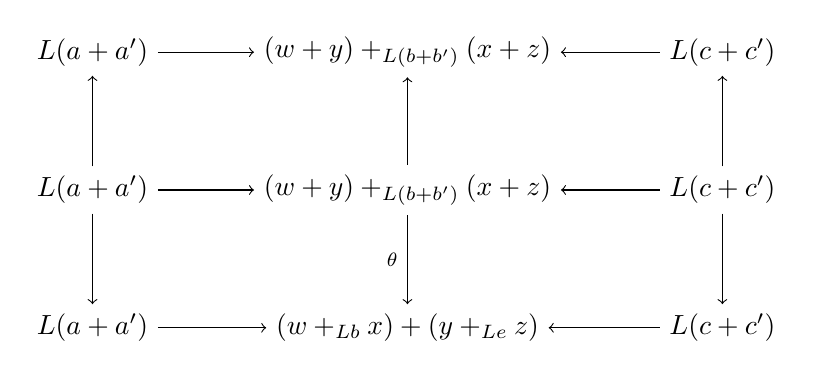
\begin{tikzpicture}
%	\draw [help lines, step=0.5, color=blue!10] (-5,-5) grid (5,5); % grid
	%
		\begin{scope}
		\node (ul) at (-4,1.75) {$ L (a + a') $};
		\node (um) at (0,1.75) {$ (w + y) +_{L (b + b')} (x + z) $};
		\node (ur) at (4,1.75) {$ L (c + c') $};
		\node (ml) at (-4,0) {$ L (a + a') $};
		\node (mm) at (0,0) {$ (w + y) +_{L (b + b')} (x + z) $};
		\node (mr) at (4,0) {$ L (c + c') $};
		\node (bl) at (-4,-1.75) {$ L ( a + a' ) $};
		\node (bm) at (0,-1.75) {$ (w+_{Lb}x) + (y+_{Le}z) $};
		\node (br) at (4,-1.75) {$ L (c + c') $};
		%
		\draw [->] (ul) to node [above] {\scriptsize $  $} (um);
		\draw [->] (ml) to node [above] {\scriptsize $  $} (mm);
		\draw [->] (bl) to node [above] {\scriptsize $  $} (bm);
		\draw [->] (ur) to node [above] {\scriptsize $  $} (um);
		\draw [->] (mr) to node [above] {\scriptsize $  $} (mm);
		\draw [->] (br) to node [above] {\scriptsize $  $} (bm);
		\draw [->] (ml) to node [left] {\scriptsize $   $} (ul);
		\draw [->] (ml) to node [left] {\scriptsize $  $} (bl);
		\draw [->] (mm) to node [left] {\scriptsize $  $} (um);
		\draw [->] (mm) to node [left] {\scriptsize $ \theta $} (bm);
		\draw [->] (mr) to node [left] {\scriptsize $  $} (ur);
		\draw [->] (mr) to node [left] {\scriptsize $  $} (br);
		\end{scope}
\end{tikzpicture}
\]
%%%%%%%%%%%%%%%%%
%%%%%%%%%%%%%%%%%
\end{document}
